%++++++++++++++++++++++++++++++++++++++++
% Don't modify this section unless you know what you're doing!
\documentclass[letterpaper, 11pt]{article}
\usepackage{tabularx} % extra features for tabular environment
\usepackage{amsmath}  % improve math presentation
\usepackage{graphicx, tipa, caption, subcaption, float, hyperref} % takes care of graphic including machinery
\usepackage[margin=1in,letterpaper]{geometry} % decreases margins
\usepackage{cite} % takes care of citations
\usepackage{comment}
\usepackage[final]{hyperref} % adds hyper links inside the generated pdf file
\usepackage{physics}
\hypersetup{
	colorlinks=true,       % false: boxed links; true: colored links
	linkcolor=blue,        % color of internal links
	citecolor=blue,        % color of links to bibliography
	filecolor=magenta,     % color of file links
	urlcolor=blue         
}
%++++++++++++++++++++++++++++++++++++++++


\begin{document}

\title{Compilation for Fast Hamiltonian Simulation \\
\large \href{https://github.com/gianelgado12/cs101-Fast-Hamiltonian-Project}{GitHub Repository}
}
\author{Wenyan Guan, Shubh Agrawal, and Gianluca Delgado}
\date{\today}
\maketitle

%\begin{abstract}
%We need an abstract.
%\end{abstract}


\section*{Project Overview}
In this project, we examined the problem of Hamiltonian simulation, which allows us to break down a Hamiltonian into a quantum circuit of elementary gates. The most established protocol in the field are the deterministic Trotter-Suzuki decompositions. Yet it has been shown that randomized compilers can achieve similarly satisfying approximation with lower computational costs. 

We studied one specific randomized Hamiltonian simulation protocol, the qDRIFT protocol by Earl Campbell \cite{PhysRevLett.123.070503}. The qDRIFT protocol weights the probability each gate proportional to the corresponding interaction strength in the Hamiltonian. Such design can eliminates the dependence of the gate count on $L$, the number of terms in the Hamiltonian and thus achieve a speed up for various practical simulations for quantum chemistry problem \cite{PhysRevLett.123.070503}.

Although we were not able to fully simulate the dynamics of hydrogen molecule due to limitation on computing power, we implemented the qDRIFT protocol in Q\# and compared its performance to that of first order Trotter-Suzuki decomposition \cite{nathanwiebe2} with several tests. Specifically, we tested the two protocols on their gate counts and total runtime varying the precision requirement $\epsilon$, terms in Hamiltonian decomposition $L$, and desired simulation time $t$.

\section*{The Hamiltonian Simulation Problem}
We formulate the Hamiltonian simulation problem formally as below. Given a Hamiltonian $H$ which decomposes into 
\begin{equation}
    H = \sum_{j = 1}^{L} h_j H_j,
\end{equation}
we would like to find a quantum circuit that approximate $e^{itH}$ as a sequence of $e^{i \tau H_j}$ gates with some precision $\varepsilon$. Moreover, we want to minimize the cost of the simulation, i.e. the number of unitaries $e^{i \tau H_j}$ used. Note that here all $H_j$'s are Hermitian and normalized.

\section*{The Trotter-Suzuki Decomposition}
The most established methods to the Hamiltonian simulation problems are currently the Trotter-Suzuki decompositions. Given a matrix exponential over matrices $A$ and $B$, the Trotter product formula
\begin{equation}
    e^{A + B} = \lim_{N \rightarrow \infty} (e^{\frac{A}{N}} e^{\frac{B}{N}})^N
\end{equation}
allows us to transform a $d$-dimensional quantum system into the corresponding $(d + 1)$-dimensional classical system \cite{SUZUKI1993432}. Generally, the Trotter-Suzuki formula $S_n$ gives the $n^{th}$ order approximation to the exponential. Here we only consider the first order formula, which simply says 
\begin{equation}
    V_r := \prod_{j = 1}^{L} e^{it h_j H_j/r} \quad \xrightarrow{ r \rightarrow \infty} \quad U_r := e^{itH/r}.
\end{equation}
It follows that $V_r^r \rightarrow U$ in large $r$ limit because $U_r^r = U$. It has been shown by previous work \cite{Childs9456} that the error for Trotter-Suzuki decomposition is bounded by
\begin{equation}
    \epsilon = \frac{L^2 \Lambda^2 t^2}{2r} e^{\frac{\Lambda t L}{r}}, \quad \Lambda := \max_{j = 1, ..., L}{h_j}.
\end{equation}
When the error $\epsilon$ is small, it is easy to see that the smallest $r$ needed $\sim \frac{L^2 \Lambda^2 t^2}{2 \epsilon}$, which brings the gate count in of the Trotter-Suzuki approximation to $N = Lr \sim \frac{L^3 \Lambda^2 t^2}{2 \epsilon}$. %As the order $n$ of the decomposition increases, the scaling approcahes $O(L^2 \Lambda t)$.
When the order of decomposition is large, the gate count roughly scales with $\order{L^2 \Lambda t}$ \cite{PhysRevLett.123.070503}. It has been noticed that there are ways to improve the $L$ dependence in the gate count\cite{Childs9456}, but never below quadratic. This imposes great limitation on the efficiency of the protocol. In fact, in chemistry problems. $L$ normally $\sim \order{n^4}$, where $n$ is the system size, which results in an unpleasant $\order{n^8}$ scaling. And the qDRIFT protocol is proposed in hope to resolve such problem.



%\section*{The qDRIFT protocol}




\section*{The qDRIFT Protocol}
% What is the logic behind your implementation?
% How did you make use of the quantum programming language?
The qDRIFT protocol leverages the power of randomized sampling to reduce the dependency on the number of terms in the Hamiltonian in the compilation of the simulation circuit. The protocol employs randomization using \textit{an oracle} (denoted $SAMPLE$) to sample from the set of unitaries that compose the full Hamiltonian. It achieves the desired precision by introducing biases into the probability distribution employed by $SAMPLE$, which is correlated to the strength of the unitaries in the full Hamiltonian expression:
\begin{equation}
    p_j = \frac{\abs{h_j}}{\sum_j \abs{h_j}},
\end{equation}
where $p_j$ is probability of $SAMPLE$ returning the unitary $H_j$. The desired precision $\epsilon$, the simulation time $t$, and the terms in decomposition $L$ together determine the number of times $N$ that $SAMPLE$ is called. Specifically, we may approximate $N$ with
\begin{equation}
    N \approx \Big\lceil \frac{2 \lambda^2 t^2}{\epsilon}\Big\rceil
\end{equation}
where $\lambda = \sum_j \abs{h_j}$. \smallskip

Each time $SAMPLE$ is called the unitary $e^{-i \tau H_j}$, where $\tau = \frac{t \lambda}{N}$, is appended to the list of unitaries to be performed in the final circuit. Here, $\frac{t}{N}$ can be thought of the time step taken ,over which the unitary is applied, in analogy to the Trotter-Suzuki decomposition; $\lambda$ is the strength of $H_j$ over that time step. We eventually obtain a final circuit with $N$ gates, where the strength of each gate is encapsulated in the number of times it appears in the circuit rather than the factor it appears along side in the exponential (which is uniform for all the gates). Thus, the length the circuit no longer explicitly depends on the number of terms in the hamiltonian decomposition $L$. One might argue that since $N$ depends on $\lambda$, $N$ does depend on $L$ indirectly, yet it can be demonstrated as in \cite{PhysRevLett.123.070503}, that for practical applications $N$ scales like $\order{L}$, which is a significant improvement from the $\order{L^2}$ barrier observed in the Trotter-Suzuki decompositions. 

The advantage qDRIFT has over higher-order trotter methods is only observable over short simulation times as qDRIFT scales like $\order{t^2}$ while higher order trotter methods scale like $\order{t}$. Thus, qDRIFT holds the most promise in simulating the dynamics of systems over a short time period with a large number of terms in their hamiltonian decompositions. 

\section*{qDRIFT Implementation}
Implement the qDRIFT protocol with the following procedures:

\begin{enumerate}
    \item Sum over the $\abs{h_j}$ values of the decomposed Hamiltonian
    \item Calculate $N$ which determines the strength of each gate in the resulting circuit
    \item Use the $SAMPLE$ oracle to sample $N$ times from the set of $H_j$ unitaries with corresponding probability $\abs{h_j}$ (suitably normalized)
    \item Append each sampled unitary to the final list of gates $V$
\end{enumerate}

Since qDRIFT does not make use of qubits to generate the circuit, we decided to implement it in Python, see \texttt{qDrift} in \texttt{host.py}. The function return the list of gates $V$ and gate count $N$ to pass on to the Q\# program, \texttt{Operations.qs}, which then perform the simulation. 

The function performing qDRIFT takes in three required (the index used to locate the Hamiltonian decomposition coefficients, the simulation time, and the desired precision) and one optional variable (the number of terms from the Hamiltonian to be used, default is set to full length of decomposition). The function then calculates $\lambda = \sum_j \abs{h_j}$, the number of gates $N$, and the probability distribution for $SAMPLE()$ in constructing the final list. An empty list $V$ is created and a for loop is used to call $SAMPLE()$ $N$ times and append a tuple of the return value of $SAMPLE()$ and $\lambda$ to $V$. Here, $SAMPLE()$ is the numpy operation \texttt{random.choice} which allows one to specify the set that is to be sampled from and the corresponding probabilities for each member of the set. The set we chose to sample from was the range of integers from zero to the number of terms the user specified to be used. These will serve as indices Q\# could then use to select the corresponding hamiltonian terms from an array specified within the Q\# program. Once the for loop has completed its execution the qDRIFT function returns the list $V$ along with the integer $N$.      

\section*{Implementing Hamiltonian Simulation}
Once the qDRIFT function has returned the list $V$ and $N$, these values are passed on to the Q\# function \texttt{sim\_ham} which takes in a list of integer-double tuples which are the index of the local hamiltonian term to be applied and its corresponding strength respectively, an integer that represents how many time steps are to be performed ($N$), and the total simulation time ($t$). \texttt{sim\_ham} then proceeds to initialize two qubits and for each element (j, $\lambda_j$) in $V$ it applies the transformation $e^{i\frac{\lambda_j t}{N} H_j}$ to the two qubits. Note this construction of the \texttt{sim\_ham} function allows one to have a different strength $\lambda_j$ for each $j$ which is taken advantage of when performing the trotter-suzuki decomposition since the strength of each $H_j$ in that case is $h_j$ which varies from term to term. For the purposes of this project the local hamiltonian terms correspond to the dynamics of the electronic structure of H2 and are hard coded at the beginning of \texttt{sim\_ham}.

\section*{Testing and Results}
% Describe the tests. Specify the output and the expected output.
In order to test the validity of our qDRIFT implementation, we compare the time it takes for qDRIFT to compile the gates and simulate the evolution to the time it takes the First Order Trotter-Suzuki method to accomplish the same task given the same simulation parameters (e.g. simulation time, target precision, Hamiltonian decomposition, etc.). We chose three metrics by which we compare the performance of qDRIFT and First Order Trotter: precision of result, number of terms, and simulation runtime.

All three types of test can be run through $\texttt{host.py}$ by using different command line arguments. The test code runs on an inputted set of Hamiltonian Decomposition Coefficients for particular $H_2$ bond lengths randomly chosen for a hard-coded list of such coefficients \texttt{H2Coeff}. The values in \texttt{H2IdentityCoeff} and \texttt{H2Terms} arrays are the corresponding Identity Transformation coefficients and 2-Local gates (0 = \texttt{Identity}, 1 = \texttt{PauliX}, 2 = \texttt{PauliY}, 3 = \texttt{PauliZ}) respectively.

The different tests along with the necessary details on running them are listed below. The code returns Usage statements if run incorrectly.
\begin{itemize}
\item 
\textbf{Precision Comparison Test. } Run \texttt{host.py} with command \texttt{python host.py 0}.

Code selects a random index \texttt{bond\_idx} representing the $H_2$ parameters. With values for logarithm of precision ranging from 0 to 2 (spacing of 0.05) and a simulation time of 1 second, simulations are run for this $H_2$ parameter set using both qDRIFT and Trotter-Suzuki protocols. The number of gates used (given by the length of \texttt{V}) and the time taken (using the \texttt{time} module) for either protocol at each log-precision value are recorded. Two plots \texttt{e\_precision\_time\_comp.png} and \texttt{e\_precision\_gates\_comp.png} are obtained from both these lists of simulation parameters.

\item 
\textbf{Number Comparison Test. } Run \texttt{host.py} with command \texttt{python host.py 1}.

Code selects a random index \texttt{bond\_idx} representing the $H_2$ parameters. With values for the number of terms in the Hamiltonian ranging from 1 to 6 (inclusive, spacing of 1) and a simulation time of 1 second, simulations are run for this $H_2$ parameter set using both qDRIFT and Trotter-Suzuki protocols. The number of gates used (given by the length of \texttt{V}) and the time taken (using the \texttt{time} module) for either protocol at each Hamiltonian count are recorded. Two plots \texttt{num\_terms\_time\_comp.png} and \texttt{num\_terms\_gates\_comp.png} are obtained from both these lists of simulation.

\item 
\textbf{Simulation Time Comparison Test. } Run \texttt{host.py} with command \texttt{python host.py 2}.

Code selects a random index \texttt{bond\_idx} representing the $H_2$ parameters. With values for the simulation time period ranging from 1 to 6 (100 points) and a log-precision of 0.1, simulations are run for this $H_2$ parameter set using both qDRIFT and Trotter-Suzuki protocols. The number of gates used (given by the length of \texttt{V}) and the time taken (using the \texttt{time} module) for either protocol at each Hamiltonian count are recorded. Two plots \texttt{sim\_time\_time\_comp.png} and \texttt{sim\_time\_gates\_comp.png} are obtained from both these lists of simulation.
\end{itemize}

These three tests were decided on for a variety of reasons. The precision test was implemented since the Campbell paper that introduces qDRIFT mostly neglects to mention how varying the precision would comparatively affect the qDRIFT and Trotter methods so it would be interesting to make such a comparison and ensure run time and gate count behave as expected given how the desired precision is used in the compilation process in both methods. Varying the simulation time also proved to be valuable as Campbell does a very similar analysis in his paper for much more complicated systems so achieving similar results on the simpler system used in this analysis should give a good indication as to whether the implementations are behaving as expected. Finally, varying the number of terms in the hamiltonian decomposition allows for the testing of Campbell's claim that qDRIFT scales much better with this variable than the Trotter methods do and this advantage should be exacerbated when comparing qDRIFT to first order Trotter. 

All three tests were run; the obtained plots (also included in the \text{Plots} of the GitHub repository) are included and analyzed below.

\subsection*{Plots with respect to precision}
\begin{figure}[H]
\centering
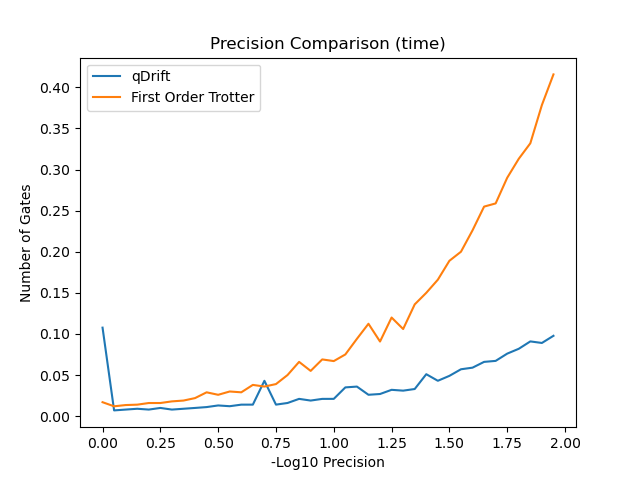
\includegraphics[width = 0.6\textwidth]{plots/e_precision_time_comp.png}
\label{html}
\caption{Linear-log space plot of the runtime with respect to the precision limit of the simulation. Note that the runtime for qDRIFT grows slower than the Trotter with respect to precision.}
\end{figure}
\begin{figure}[H]
\centering
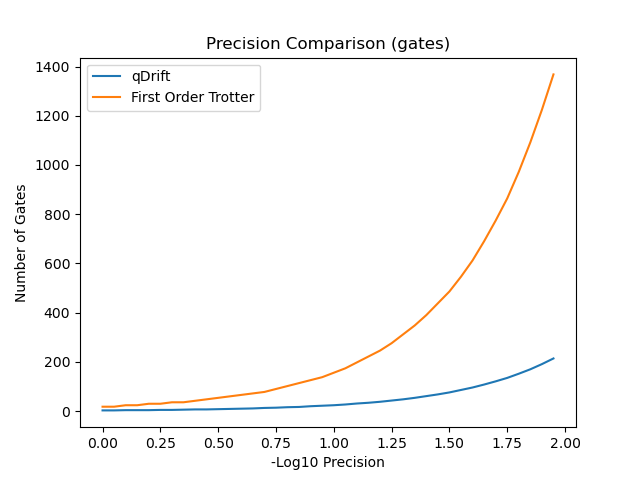
\includegraphics[width = 0.6\textwidth]{plots/e_precision_gates_comp.png}
\label{html}
\caption{Linear-log space plot of the number of Quantum gates needed for the precision limit of the simulation. Note that this number of gates, which represents the circuit complexity, grows slower for qDRIFT than the Trotter with respect to precision. The curve is also much smoother than that for the runtime, as expected, due to less noise associated with the deterministic process for choosing gates.}
\end{figure}

\subsection*{Plots with respect to number of Hamiltonian terms}
\begin{figure}[H]
\centering
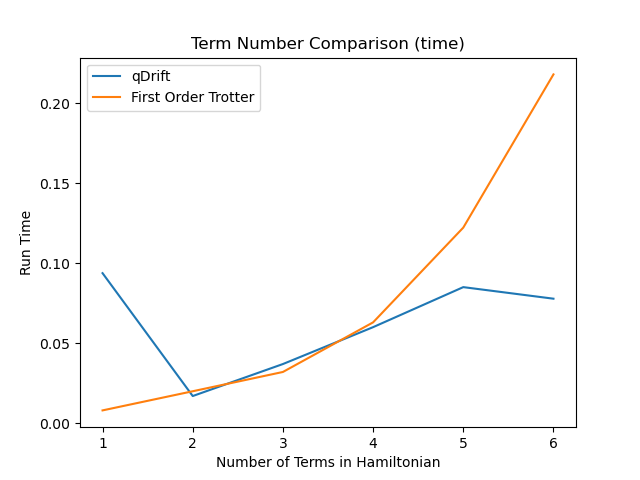
\includegraphics[width = 0.6\textwidth]{plots/num_terms_time_comp.png}
\label{html}
\caption{Linear space plot of the runtime with respect to the number of terms in the Hamiltonian being simulated. Note that the runtime for qDRIFT grows slower than the Trotter with respect to the Hamiltonian length, though is much less observable than the other two tests due to the smaller range of independent variable (number of terms) values.}
\end{figure}
\begin{figure}[H]
\centering
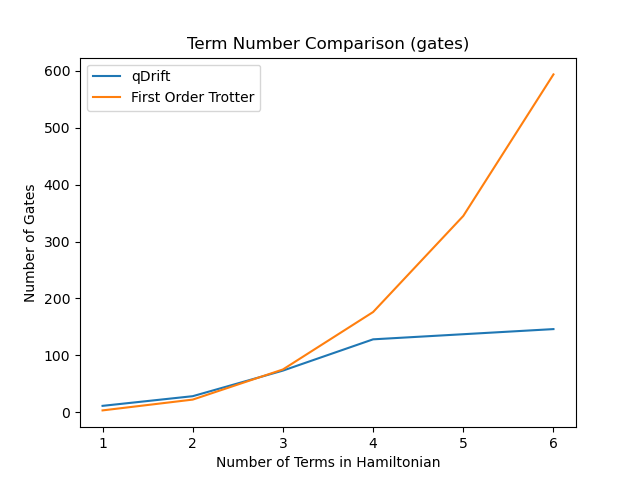
\includegraphics[width = 0.6\textwidth]{plots/num_terms_gates_comp.png}
\label{html}
\caption{Linear space plot of the number of gates needed (representing circuit complexity) with respect to the number of terms in the Hamiltonian being simulated. Note that the complexity for qDRIFT seems to grow slower than the Trotter with respect to Hamiltonian length.}
\end{figure}

\subsection*{Plots with respect to simulation time period}
\begin{figure}[H]
\centering
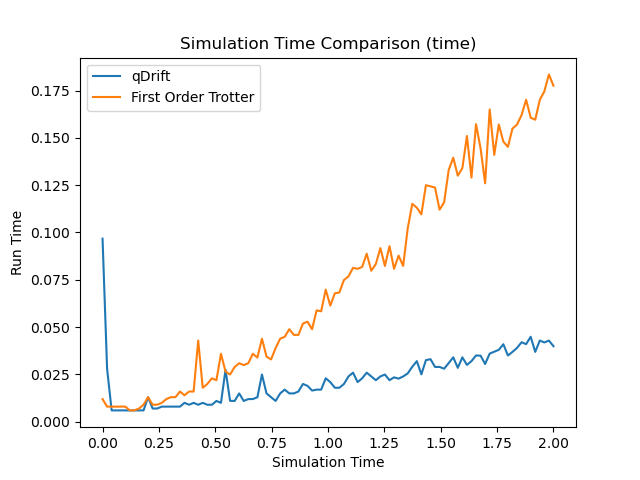
\includegraphics[width = 0.6\textwidth]{plots/sim_time_time_comp.png}
\label{html}
\caption{Linear space plot of the runtime with respect to the time period for which the system is simulated. Note that the runtime for qDRIFT again grows slower than the Trotter with respect to simulation time. There is much more noise associated with the data due to the more dense range of independent variable.}
\end{figure}
\begin{figure}[H]
\centering
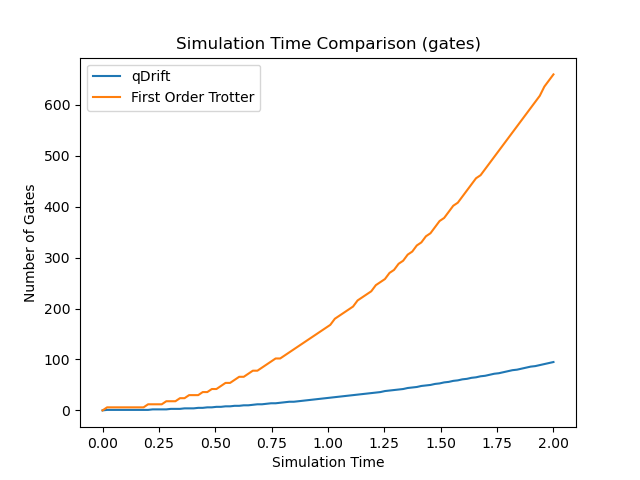
\includegraphics[width = 0.6\textwidth]{plots/sim_time_gates_comp.png}
\label{html}
\caption{Linear space plot of the number of terms in the circuit with respect to the time period for which the system is simulated. Note that this circuit complexity grows slower for qDRIFT than the Trotter with respect to simulation time. The curve is also much smoother than that for the runtime, as expected, due to less noise associated with the deterministic process for choosing gates.}
\end{figure}


% \begin{comment}


% \bigskip
% \begin{figure}[ht] 
%         % read manual to see what [ht] means and for other possible options
%         \centering \includegraphics[width=0.8\columnwidth]{sr_setup}
%         % note that in above figure file name, "sr_setup",
%         % the file extension is missing. LaTeX is smart enough to find
%         % apropriate one (i.e. pdf, png, etc.)
%         % You can add this extention yourself as it seen below
%         % both notations are correct but above has more flexibility
%         %\includegraphics[width=1.0\columnwidth]{sr_setup.pdf}
%         \caption{
%                 \label{fig:samplesetup} % spaces are big no-no withing labels
%                 % things like fig: are optional in the label but it helps
%                 % to orient yourself when you have multiple figures,
%                 % equations and tables
%                 Every figure MUST have a caption.
%         }
% \end{figure}

% Don't forget to list all important steps in your experimental procedure!

% Use active voice either in past or present through all the report and be
% consistent with it:
% The laser light comes  from to ... and eventually arrived to the
% balanced photodiode as seen in the figure~\ref{fig:samplesetup}.

% Sentences in the past voice while correct are generally considered hard to read
% in large numbers. The laser light was directed to ..., wave plates were set
% to ... etc.


% %\section*{Results and Analysis}
% What result did you obtain?
% Do they match the expected results?

% In this section you will need to show your experimental results. Use tables and
% graphs when it is possible. Table~\ref{tbl:bins} is an example.

% \begin{table}[ht]
% \begin{center}
% \caption{Every table needs a caption.}
% \label{tbl:bins} % spaces are big no-no withing labels
% \begin{tabular}{|cc|} 
% \hline
% \multicolumn{1}{|c}{$x$ (m)} & \multicolumn{1}{c|}{$V$ (V)} \\
% \hline
% 0.0044151 &   0.0030871 \\
% 0.0021633 &   0.0021343 \\
% 0.0003600 &   0.0018642 \\
% 0.0023831 &   0.0013287 \\
% \hline
% \end{tabular}
% \end{center}
% \end{table}

% Analysis of equation~\ref{eq:aperp} shows ...

% Note: this section can be integrated with the previous one as long as you
% address the issue. Here explain how you determine uncertainties for different
% measured values. Suppose that in the experiment you make a series of
% measurements of a resistance of the wire $R$ for different applied voltages
% $V$, then you calculate the temperature from the resistance using a known
% equation and make a plot  temperature vs. voltage squared. Again suppose that
% this dependence is expected to be linear~\cite{Cyr}, and the proportionality coefficient
% is extracted from the graph. Then what you need to explain is that for the
% resistance and the voltage the uncertainties are instrumental (since each
% measurements in done only once), and they are $\dots$. Then give an equation
% for calculating the uncertainty of the temperature from the resistance
% uncertainty. Finally explain how the uncertainty of the slop of the graph was
% found (computer fitting, graphical method, \emph{etc}.)

% If in the process of data analysis you found any noticeable systematic
% error(s), you have to explain them in this section of the report.

% It is also recommended to plot the data graphically to efficiently illustrate
% any points of discussion. For example, it is easy to conclude that the
% experiment and theory match each other rather well if you look at
% Fig.~\ref{fig:samplesetup} and Fig.~\ref{fig:exp_plots}.

% \begin{figure}[ht] 
%   \centering
%       \includegraphics[width=0.5\columnwidth]{sr_squeezing_vs_detuning}

% % some figures do not need to be too wide
%         \caption{
%                 \label{fig:exp_plots}  
%                 Every plot must have axes labeled.
%         }
% \end{figure}

% \end{comment}

\section*{Summary}
In general, it is noted from all three tests than both the time complexity and circuit complexity scale faster (with respect to any of the initial state parameters) for the first order Trotter than for the qDRIFT protocol.

%++++++++++++++++++++++++++++++++++++++++
% References section will be created automatically 
% with inclusion of "thebibliography" environment
% as it shown below. See text starting with line
% \begin{thebibliography}{99}
% Note: with this approach it is YOUR responsibility to put them in order
% of appearance.

\bibliographystyle{ieeetr}
\bibliography{bibfile.bib}


%\begin{thebibliography}{99}

%\bibitem{melissinos}
%A.~C. Melissinos and J. Napolitano, \textit{Experiments in Modern Physics},
%(Academic Press, New York, 2003).

%\bibitem{Cyr}
%N.\ Cyr, M.\ T$\hat{e}$tu, and M.\ Breton,
% "All-optical microwave frequency standard: a proposal,"
%IEEE Trans.\ Instrum.\ Meas.\ \textbf{42}, 640 (1993).

%\bibitem{Wiki} \emph{Expected value},  available at
%\texttt{http://en.wikipedia.org/wiki/Expected\_value}.

%\end{thebibliography}


\end{document}
